\documentclass[10pt,letterpaper,titlepage]{report}
\usepackage{algorithm2e}
\usepackage{hyperref}
\usepackage{listings}
\usepackage{geometry}
\usepackage{graphicx}

% use pdflatex ParallelDetails.tex
%%%%%%%%%%%%%%%%%%%%%%%%%%%%%%%%%%%%%%%%%%%%%%%%%%%%%%%%%%%%%%%%%%%%
%%%%%%%%%%%%%%%%%%%%%%%%%%%%%%%%%%%%%%%%%%%%%%%%%%%%%%%%%%%%%%%%%%%%

\author{Berenger Bramas}
\title{ScalFmm - Parallel Algorithms (Draft)}
\date{August, 2011}

\lstset{language=c++, frame=lines}

%% ou \addtolength{\voffset}{-1.5cm} \addtolength{\textheight}{2cm}
%% \addtolength{\hoffset}{-1cm} \addtolength{\textwidth}{2cm}
\geometry{scale=0.8, nohead}

\setcounter{secnumdepth}{-1}

\begin{document}
\maketitle{}
\newpage

\tableofcontents
\newpage

%%%%%%%%%%%%%%%%%%%%%%%%%%%%%%%%%%%%%%%%%%%%%%%%%%%%%%%%%%%%%%%%%%%%
%%%%%%%%%%%%%%%%%%%%%%%%%%%%%%%%%%%%%%%%%%%%%%%%%%%%%%%%%%%%%%%%%%%%

\section{Introduction}
In this document we introduce the principles and the algorithms used in our library to run in a distributed environment using MPI.
The algorithms in this document may not be up to date comparing to those used in the code.
We advice to check the version of this document and the code to have the lastest available.

%%%%%%%%%%%%%%%%%%%%%%%%%%%%%%%%%%%%%%%%%%%%%%%%%%%%%%%%%%%%%%%%%%%%
%%%%%%%%%%%%%%%%%%%%%%%%%%%%%%%%%%%%%%%%%%%%%%%%%%%%%%%%%%%%%%%%%%%%

\chapter{Building the tree in Parallel}
\section{Description}
The main motivation to create a distributed version of the FMM is to run large simulation.
These simulations contains more particles than a computer can host which involves to use several computers.
Moreover, that is the reason why it is not reasonable to ask a master process to load an entire file and to dispatch the data to others processes. Without being able to know the entire tree it may send randomly the data to the slaves.

To override this situation, we use a solution that can be viewed as a two steps process.
First, each node loads a part of the file to possess several particles.
After this task, each node can compute the Morton index for the particles he loaded.
The Morton index of a particle depends of the system properties but also of the tree height.
If we want to choose the tree height and the number of nodes at run time then we cannot pre-process the file.
The second step is a parallel sort based on the Morton index between all nodes with a balancing operation at the end.

%%%%%%%%%%%%%%%%%%%%%%%%%%%%%%%%%%%%%%%%%%%%%%%%%%%%%%%%%%%%%%%%%%%%
%%%%%%%%%%%%%%%%%%%%%%%%%%%%%%%%%%%%%%%%%%%%%%%%%%%%%%%%%%%%%%%%%%%%

\section{Load a file in parallel}
We use the MPI $I/O$ functions to split a file between all the mpi processes.
The prerequisite to make the spliting easier is to have a binary file.
Thereby, using a very basic formula each node know which part of the file it needs to load.

\begin{equation}
size per proc \leftarrow \left (file size - header size \right ) / nbprocs
\end{equation}
\begin{equation}
offset \leftarrow header size + size per proc .\left ( rank - 1 \right )
\end{equation}
\newline

The MPI $I/O$ functions use a view model to manage data access.
We first construct a view using the function MPI\_File\_set\_view and then read the data with MPI\_File\_read as described in the fallowing $C++$ code.

\begin{lstlisting}
// From FMpiFmaLoader
particles = new FReal[bufsize];
MPI_File_set_view(file, headDataOffSet + startPart * 4 * sizeof(FReal),
	MPI_FLOAT, MPI_FLOAT, const_cast<char*>("native"), MPI_INFO_NULL);
MPI_File_read(file, particles, bufsize, MPI_FLOAT, &status);
\end{lstlisting}

Our files are composed by a header fallowing by all the particles.
The header enable to check the precision of the file.
Finally, a particles is represented by four values: a position and a physical value.

%%%%%%%%%%%%%%%%%%%%%%%%%%%%%%%%%%%%%%%%%%%%%%%%%%%%%%%%%%%%%%%%%%%%
%%%%%%%%%%%%%%%%%%%%%%%%%%%%%%%%%%%%%%%%%%%%%%%%%%%%%%%%%%%%%%%%%%%%

\section{Sorting the particles}
Once each node has a set of particles we need to sort them.
This problem boils down to a simple parallel sort where Morton index are used to compare particles.

\subsection{Using QuickSort}
A first approach is to use a famous sorting algorithm.
We choose to use the quick sort algorithm because the distributed and the shared momory approches are mostly similar.
Our implementation is based on the implementation describe in \cite{itpc03}.
The efficiency of this algorithm depends roughly of the pivot choice.
In fact, a wrong idea of the parallel quick sort is to think that each process first sort their particles and second use a merge sort to share their results.
Instead, the nodes choose a pivot and do one quick sort iteration together.
From that point all process has an array with a left part where all value are lower than the pivot and a right part where all values are upper or equal than the pivot.
Then, the nodes exchange data and some of them will work on the lower part and the other on the upper parts until there is one process for a part.
At this point, the process perform a shared memory quick sort.
To choose the pivot we tried to use an average of all the data hosted by the nodes:
\newline

\begin{algorithm}[H]
\SetLine
\KwResult{A Morton index as next iteration pivot}
\BlankLine
myFirstIndex $\leftarrow$ particles$[0]$.index\;
allFirstIndexes $\leftarrow$ MortonIndex$[nbprocs]$\;
allGather(myFirstIndex, allFirstIndexes)\;
pivot $\leftarrow$ Sum(allFirstIndexes) / nbprocs\;
\BlankLine
\caption{Choosing the QS pivot}
\end{algorithm}

%%%%%%%%%%%%%%%%%%%%%%%%%%%%%%%%%%%%%%%%%%%%%%%%%%%%%%%%%%%%%%%%%%%%
%%%%%%%%%%%%%%%%%%%%%%%%%%%%%%%%%%%%%%%%%%%%%%%%%%%%%%%%%%%%%%%%%%%%

\subsection{Using an intermediate Octree}
The second approach uses an octree to sort the particles in each process instead of a sorting algorithm.
The time complexity is equivalent but it needs more memory since it is not done in place.
After inserting the particles in the tree, we can iterate at the leaves level and access to the particles in an ordered way.
Then, the processes are doing a minimum and a maximum reduction to know the real Morton interval of the system.
By building the system interval in term of Morton index, the nodes cannot know the data scattering.
Finally, the processes split the interval in a uniform manner and exchange data with $P^{2}$ communication in the worse case.
\newline
\newline
In both approaches the data may not be balanced at the end.
In fact, the first method is pivot dependant and the second consider that the data are uniform.
That is the reason why we need to balance the data among nodes.

%%%%%%%%%%%%%%%%%%%%%%%%%%%%%%%%%%%%%%%%%%%%%%%%%%%%%%%%%%%%%%%%%%%%
%%%%%%%%%%%%%%%%%%%%%%%%%%%%%%%%%%%%%%%%%%%%%%%%%%%%%%%%%%%%%%%%%%%%

\section{Balancing the leaves}
After sorting, each process has potentialy several leaves.
If we have to processes $P_{i}$ and $P_{j}$ with $i < j$ the sort guarantes that all leaves from node i are inferior than the leaves on the node j in a Morton indexing way.
But the leaves are randomly distributed among the nodes and we need to balance them.
Our idea is to use a two passes algorithm describes as a sand settling:
\begin{enumerate}
\item We can see each node as a heap of sand.
This heap represents the leaves of the octree.
Some nodes have lot of leaves and then have a big heaps.
On the contraray, some other have small heaps.
Starting from the extremities, each node can know the sand there is on its left and on its right.
\item Because each node knows the total among of sand in the system which is the sum of the sand there is on each of its sides plus its own sand it can compute a balancing calculs.
What should happen if we put a heavy plank above all our sand heaps?
Well the system should balance until all heaps have the same size.
The same happens here, each node can know what to do to balance the system.
Each node communicate only with its two neighbors by sending or receiving entire leaves.
\end{enumerate}

At the end of the algorithm our system is completly balanced with the same number of leaves on each processes.


\begin{figure}[h!]
\begin{center}
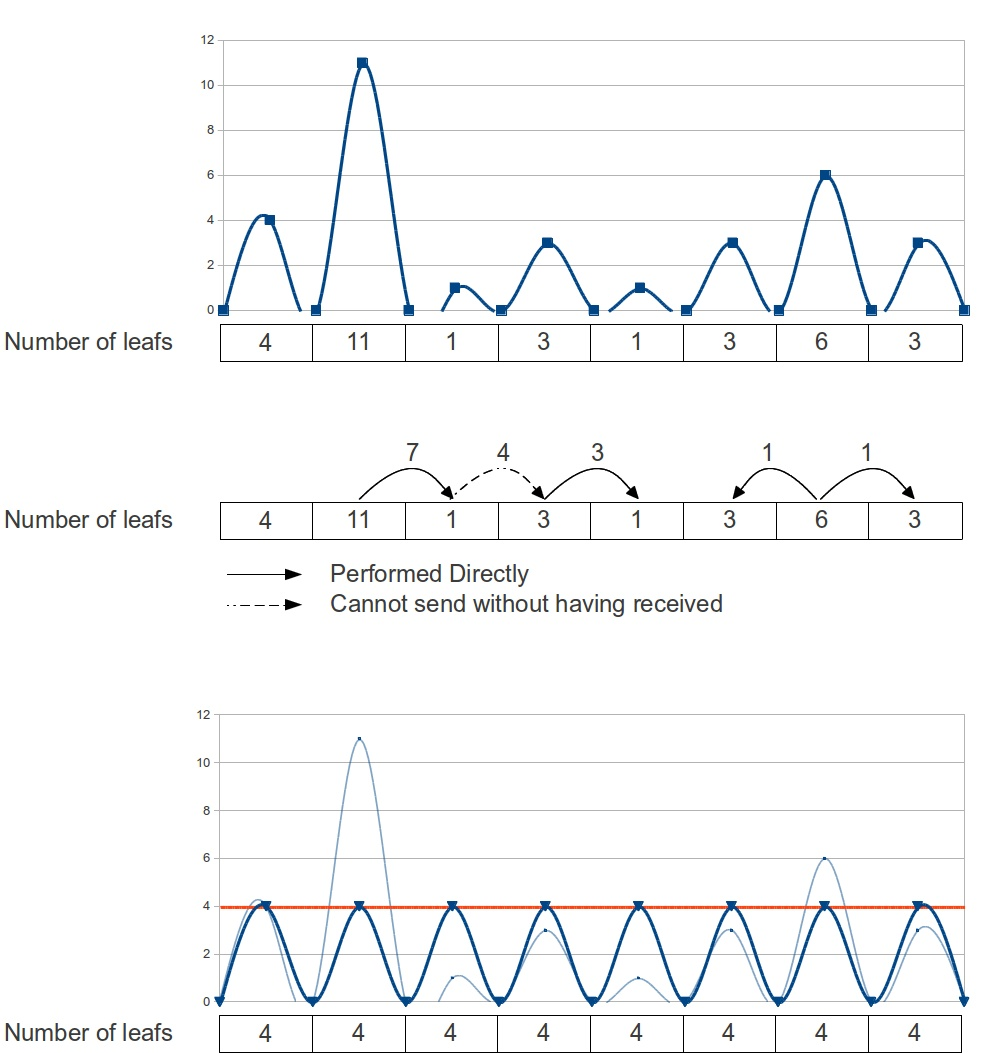
\includegraphics[width=15cm, height=20cm, keepaspectratio=true]{SandSettling.png} 
\caption{Sand Settling Example}
\end{center}
\end{figure}

%%%%%%%%%%%%%%%%%%%%%%%%%%%%%%%%%%%%%%%%%%%%%%%%%%%%%%%%%%%%%%%%%%%%
%%%%%%%%%%%%%%%%%%%%%%%%%%%%%%%%%%%%%%%%%%%%%%%%%%%%%%%%%%%%%%%%%%%%

\chapter{Simple operators: P2M, M2M, L2L}
We present the different FMM operators in two separated parts depending on their parallel complexity.
In this first part we present the three simpliest operators P2M, M2M and L2L.
Their simplicity is explain by the possible prediction to know which node hosts a cell and how to organized the communication.

\section{P2M}
The P2M still unchanged from the sequential approach to the distributed memory algorithm.
In fact, in the sequential model we compute a P2M between all particles of a leaf and this same leaf which is also a cell.
Although, a leaf and the particles it hosts belong to only one node so doing the P2M operator do not require any information from another node.
From that point, using the shared memory operator makes sense.

%%%%%%%%%%%%%%%%%%%%%%%%%%%%%%%%%%%%%%%%%%%%%%%%%%%%%%%%%%%%%%%%%%%%
%%%%%%%%%%%%%%%%%%%%%%%%%%%%%%%%%%%%%%%%%%%%%%%%%%%%%%%%%%%%%%%%%%%%

\section{M2M}
During the upward pass information moves from a level to the upper one.
The problem in a distributed memory model is that one cell can exist in several trees i.e. in several nodes.
Because the M2M operator compute the relation between a cell and its child, the nodes which have a cell in commom need to share information.
Moreover, we have to decide which process will be responsible of the computation if the cell is present on more than one node.

We have decided that the node with the smallest rank has the responsibility to compute the M2M and propagate the value for the future operations.
Despite the fact that others processes are not computing this cell, they have to send the child of this shared cell to the responsible node.

Concentring on that problem enable to establish some rules.
In fact, at each iteration a process never needs to send more than 8-1 cells, also a process never needs to receive more than 8-1 cells.
Also, the shared cells are always at extremities and one process cannot be designed to be the responsible of more than one shared cell at a level.


\begin{algorithm}[H]
\SetLine
\KwData{none}
\KwResult{none}
\BlankLine
\For{idxLevel $\leftarrow$ $Height - 2$ \KwTo 1}{
	\ForAll{Cell c at level idxLevel}{
		M2M(c, c.child)\;
	}
}
\BlankLine
\caption{Traditional M2M}
\end{algorithm}


\begin{algorithm}[H]
\SetLine
\KwData{none}
\KwResult{none}
\BlankLine
\For{idxLevel $\leftarrow$ $Height - 2$ \KwTo 1}{
	\uIf{$cells[0]$ not in my working interval}{
		isend($cells[0].child$)\;
		hasSend $\leftarrow$ true\;
	}
	\uIf{$cells[end]$ in another working interval}{
		irecv(recvBuffer)\;
		hasRecv $\leftarrow$ true\;
	}
	\ForAll{Cell c at level idxLevel in working interval}{
		M2M(c, c.child)\;
	}
	\emph{Wait send and recv if needed}\;
	\uIf{hasRecv is true}{
		M2M($cells[end]$, recvBuffer)\;
	}
}
\BlankLine
\caption{Distributed M2M}
\end{algorithm}

%%%%%%%%%%%%%%%%%%%%%%%%%%%%%%%%%%%%%%%%%%%%%%%%%%%%%%%%%%%%%%%%%%%%
%%%%%%%%%%%%%%%%%%%%%%%%%%%%%%%%%%%%%%%%%%%%%%%%%%%%%%%%%%%%%%%%%%%%

\section{L2L}
The L2L operator is very similar to the M2M.
On the contrary that a result hosted by only one node need to be shared with every other nodes that are responsible of some child of this node.

\begin{algorithm}[H]
\SetLine
\KwData{none}
\KwResult{none}
\BlankLine
\For{idxLevel $\leftarrow$ 2 \KwTo $Height - 2$ }{
	\uIf{$cells[0]$ not in my working interval}{
		irecv($cells[0]$)\;
		hasRecv $\leftarrow$ true\;
	}
	\uIf{$cells[end]$ in another working interval}{
		isend($cells[end]$)\;
		hasSend $\leftarrow$ true\;
	}
	\ForAll{Cell c at level idxLevel in working interval}{
		M2M(c, c.child)\;
	}
	\emph{Wait send and recv if needed}\;
	\uIf{hasRecv is true}{
		M2M($cells[0]$, $cells[0].child$)\;
	}
}
\BlankLine
\caption{Distributed L2L}
\end{algorithm}

%%%%%%%%%%%%%%%%%%%%%%%%%%%%%%%%%%%%%%%%%%%%%%%%%%%%%%%%%%%%%%%%%%%%
%%%%%%%%%%%%%%%%%%%%%%%%%%%%%%%%%%%%%%%%%%%%%%%%%%%%%%%%%%%%%%%%%%%%

\chapter{Complex operators: P2P, M2L}
This two operators are more complex than the ones presented in the previous chapter.
In fact, they require a gather and a pre-process task that take time.

\section{P2P}
To process the P2P we need the neighbors of all our leaves.
But this neighbors can be potentially hosted by any other process because of the Morton indexing.
Also, our tree is an indirection tree, so a leaf may not exist because there is particles at this place.
From that description of the problem we have implemented the fallowing algorithm.

\begin{algorithm}[H]
\SetLine
\KwData{none}
\KwResult{none}
\BlankLine

\ForAll{Leaf lf}{
	neighborsIndexes $\leftarrow$ $lf.potentialNeighbors()$\;
	\ForAll{index in neighborsIndexes}{
		\uIf{index belong to another proc}{
			isend(lf)\;
			\emph{Mark lf as a leaf that is linked to another proc}\;
		}
	}
}
\emph{all gather how many particles to send to who}\;
\emph{prepare the buffer to receive data}\;
\ForAll{Leaf lf}{
	\uIf{lf is not linked to another proc}{
		neighbors $\leftarrow$ $tree.getNeighbors(lf)$\;
		P2P(lf, neighbors)\;
	}
}
\emph{Wait send and recv if needed}\;
\emph{Put received particles in a fake tree}\;
\ForAll{Leaf lf}{
	\uIf{lf is linked to another proc}{
		neighbors $\leftarrow$ $tree.getNeighbors(lf)$\;
		otherNeighbors $\leftarrow$ $fakeTree.getNeighbors(lf)$\;
		P2P(lf, neighbors + otherNeighbors)\;
	}
}

\BlankLine
\caption{Distributed P2P}
\end{algorithm}

%%%%%%%%%%%%%%%%%%%%%%%%%%%%%%%%%%%%%%%%%%%%%%%%%%%%%%%%%%%%%%%%%%%%
%%%%%%%%%%%%%%%%%%%%%%%%%%%%%%%%%%%%%%%%%%%%%%%%%%%%%%%%%%%%%%%%%%%%

\section{M2L}
The M2L operator is relatively similar to the P2P.
Hence P2P is done at the leaves level, M2L is done from several levels from Height - 2 to 2.
At each level we need to have access to neighbors of the cells we are proprietary and those ones can be hosted by any processes.
But we can process most of the cells without the need of data from other processes.
That is the reason why we work with several tasks:
\begin{enumerate}
\item Compute to know what data has to be sent
\item Do all the computation we can without the data from others
\item Wait sendings and receptions
\item Compute M2L with the data we received
\end{enumerate}

Then the algorithm is detailled in the fallowing figure:

\begin{algorithm}[H]
\SetLine
\KwData{none}
\KwResult{none}
\BlankLine
\ForAll{Level idxLeve from 2 to Height - 2}{
	\ForAll{Cell c at level idxLevel}{
		neighborsIndexes $\leftarrow$ $c.potentialDistantNeighbors()$\;
		\ForAll{index in neighborsIndexes}{
			\uIf{index belong to another proc}{
				isend(c)\;
				\emph{Mark c as a cell that is linked to another proc}\;
			}
		}
	}
}
\emph{Normal M2L}\;
\emph{Wait send and recv if needed}\;
\ForAll{Cell c received}{
	$lightOctree.insert( c )$\;
}
\ForAll{Level idxLeve from 2 to Height - 2}{
	\ForAll{Cell c at level idxLevel that are marked}{
		neighborsIndexes $\leftarrow$ $c.potentialDistantNeighbors()$\;
		neighbors $\leftarrow$ lightOctree.get(neighborsIndexes)\;
		M2L( c, neighbors)\;
	}
}
\BlankLine
\caption{Distributed M2L}
\end{algorithm}

%%%%%%%%%%%%%%%%%%%%%%%%%%%%%%%%%%%%%%%%%%%%%%%%%%%%%%%%%%%%%%%%%%%%
%%%%%%%%%%%%%%%%%%%%%%%%%%%%%%%%%%%%%%%%%%%%%%%%%%%%%%%%%%%%%%%%%%%%

\begin{thebibliography}{9}

\bibitem{itpc03}
   Ananth Grama, George Karypis, Vipin Kumar, Anshul Gupta,
   \emph{Introduction to Parallel Computing}.
   Addison Wesley, Massachusetts,
   2nd Edition,
   2003.

\end{thebibliography}

\end{document}
